% Created 2024-02-27 Tue 15:14
% Intended LaTeX compiler: pdflatex
\documentclass[presentation,10pt]{beamer}
\usepackage[utf8]{inputenc}
\usepackage[T1]{fontenc}
\usepackage{graphicx}
\usepackage{longtable}
\usepackage{wrapfig}
\usepackage{rotating}
\usepackage[normalem]{ulem}
\usepackage{amsmath}
\usepackage{amssymb}
\usepackage{capt-of}
\usepackage{hyperref}
\mode<beamer>{\usetheme{Madrid}}
\definecolor{SUred}{rgb}{0.59375, 0, 0.17969} % SU red (primary)
\definecolor{SUblue}{rgb}{0, 0.17578, 0.38281} % SU blue (secondary)
\setbeamercolor{palette primary}{bg=SUred,fg=white}
\setbeamercolor{palette secondary}{bg=SUblue,fg=white}
\setbeamercolor{palette tertiary}{bg=SUblue,fg=white}
\setbeamercolor{palette quaternary}{bg=SUblue,fg=white}
\setbeamercolor{structure}{fg=SUblue} % itemize, enumerate, etc
\setbeamercolor{section in toc}{fg=SUblue} % TOC sections
% Override palette coloring with secondary
\setbeamercolor{subsection in head/foot}{bg=SUblue,fg=white}
\setbeamercolor{date in head/foot}{bg=SUblue,fg=white}
\institute[SU]{Shenandoah University}
\titlegraphic{\includegraphics[width=0.5\textwidth]{\string~/Documents/suLogo/suLogo.pdf}}
\newcommand{\R}{\mathbb{R}}
\usepackage{tikz}
\usetheme{default}
\author{Chase Mathison\thanks{cmathiso@su.edu}}
\date{28 February 2024}
\title{Graphing the other Trig Functions}
\hypersetup{
 pdfauthor={Chase Mathison},
 pdftitle={Graphing the other Trig Functions},
 pdfkeywords={},
 pdfsubject={},
 pdfcreator={Emacs 29.1 (Org mode 9.6.7)}, 
 pdflang={English}}
\begin{document}

\maketitle

\section{Announcements}
\label{sec:orgda88200}
\begin{frame}[label={sec:org0c28fdf}]{Announcements}
\begin{enumerate}
\item Homework in Canvas.
\item Exam Corrections due in 1 week.
\item Office hours today: 10am - 11am.
\end{enumerate}
\end{frame}

\section{Lecture}
\label{sec:org12ba74a}
\begin{frame}[label={sec:orgd7dc76d}]{The Graphs of the other Trig Functions}
Let's start class with some boring tables:
\end{frame}

\begin{frame}[label={sec:orgacc7cb7}]{The Graphs of the other Trig Functions}
\begin{center}
\begin{tabular}{|c|c|c|c|c|}
\hline
\(x\) & \(\tan(x)\) & \(\cot(x)\) & \(\sec(x)\) & \(\csc\)(x)\\[0pt]
\hline
\(-\pi\) &  &  &  & \\[0pt]
\hline
\(-5\pi/6\) &  &  &  & \\[0pt]
\hline
\(-3\pi/4\) &  &  &  & \\[0pt]
\hline
\(-2\pi/3\) &  &  &  & \\[0pt]
\hline
\(-\pi/2\) &  &  &  & \\[0pt]
\hline
\(-\pi/3\) &  &  &  & \\[0pt]
\hline
\(-\pi/4\) &  &  &  & \\[0pt]
\hline
\(-\pi/6\) &  &  &  & \\[0pt]
\hline
0 &  &  &  & \\[0pt]
\hline
\(\pi/6\) &  &  &  & \\[0pt]
\hline
\(\pi/4\) &  &  &  & \\[0pt]
\hline
\(\pi/3\) &  &  &  & \\[0pt]
\hline
\(\pi/2\) &  &  &  & \\[0pt]
\hline
\(2\pi/3\) &  &  &  & \\[0pt]
\hline
\(3\pi/4\) &  &  &  & \\[0pt]
\hline
\(5\pi/6\) &  &  &  & \\[0pt]
\hline
\(\pi\) &  &  &  & \\[0pt]
\hline
\end{tabular}
\end{center}
\end{frame}

\begin{frame}[label={sec:orgdc97da2}]{Graphing variations of tangent: \(A \tan (Bx - C) + D\)}
\begin{center}
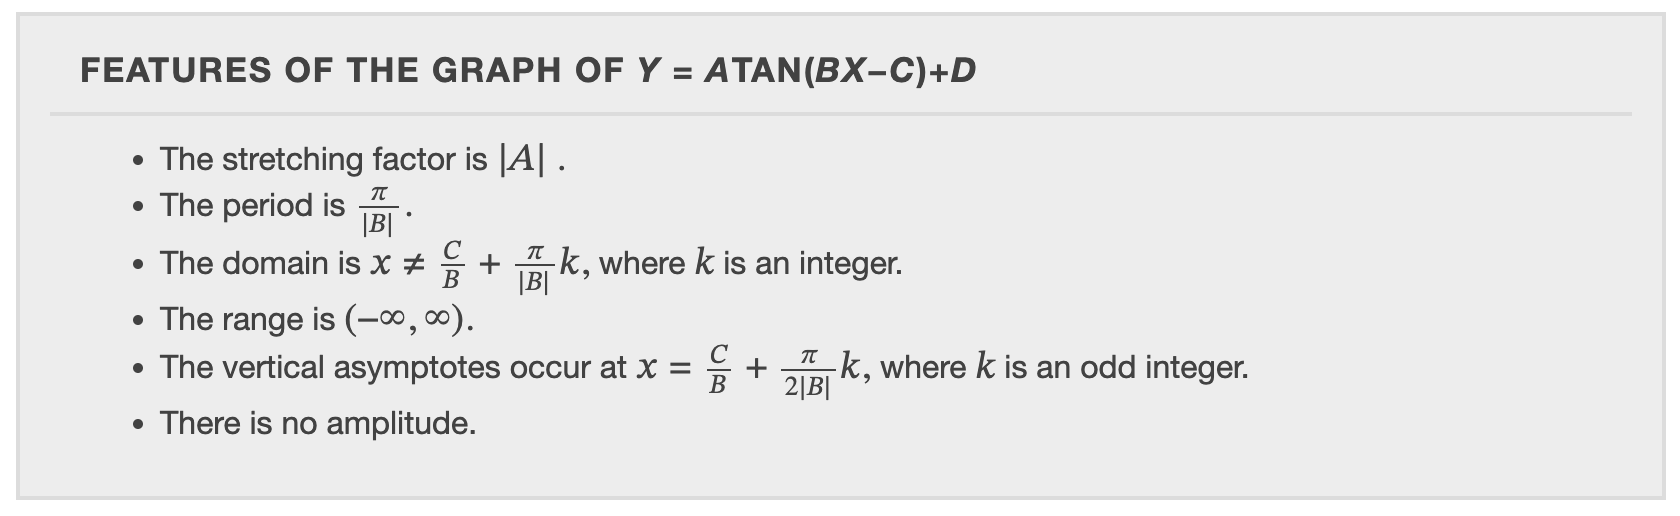
\includegraphics[width=0.9\textwidth]{./tanFeat.png}
\end{center}


\begin{center}
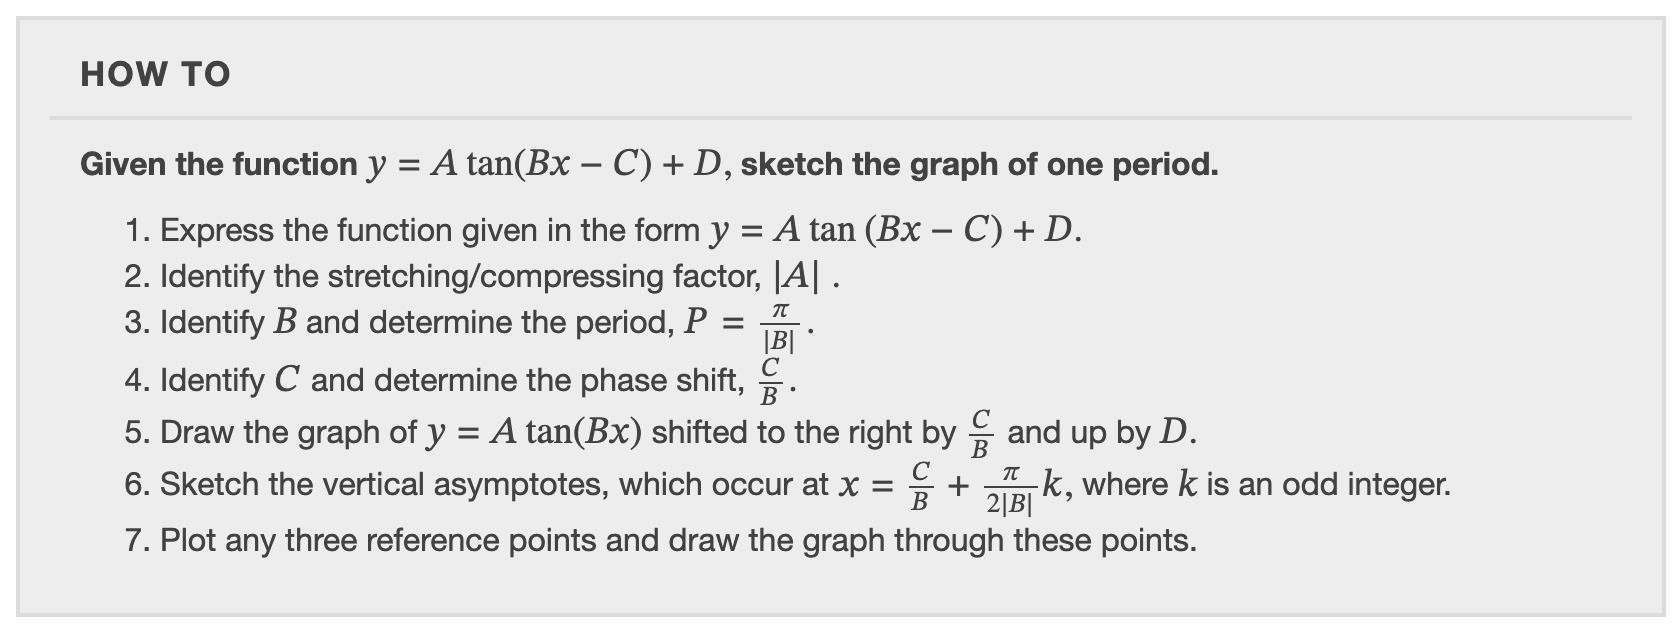
\includegraphics[width=0.9\textwidth]{./howToTan.png}
\end{center}
\end{frame}


\begin{frame}[label={sec:orgeaec6f9}]{Graphing variations of secant: \(A \sec (Bx - C) + D\)}
\begin{center}
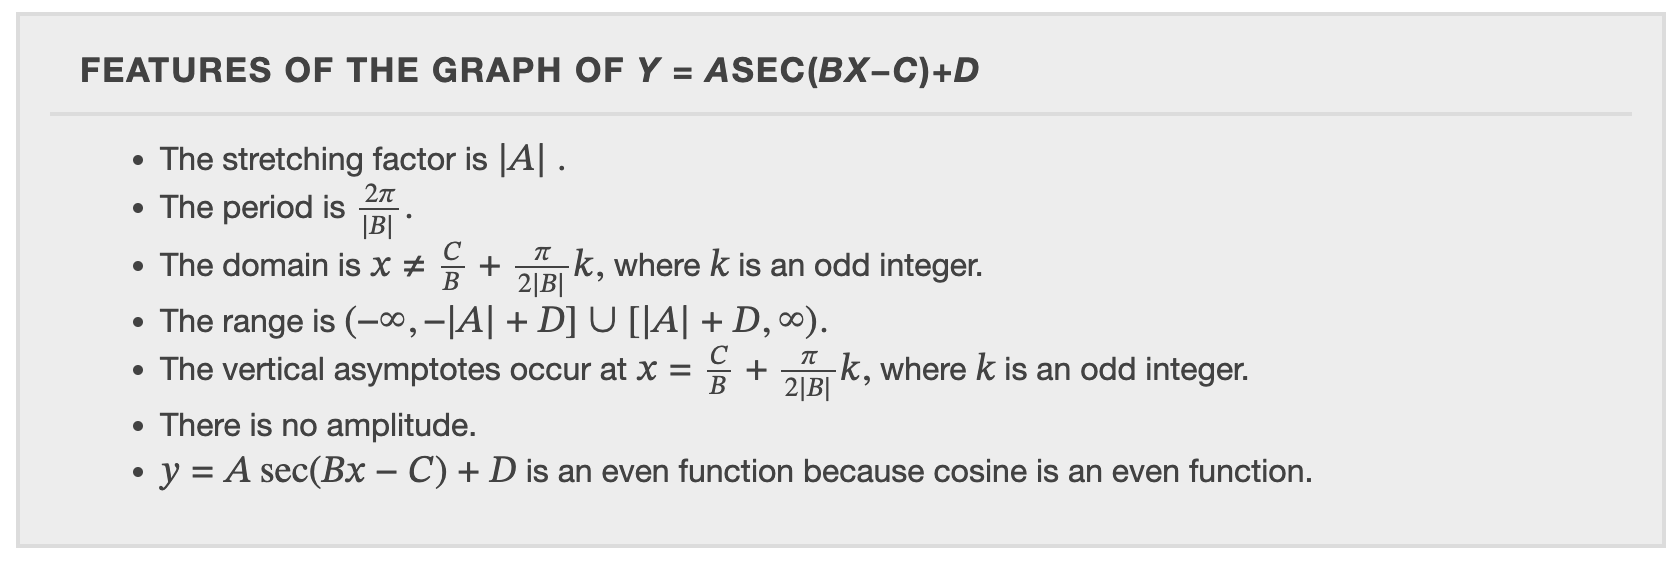
\includegraphics[width=0.9\textwidth]{./secFeat.png}
\end{center}

\begin{center}
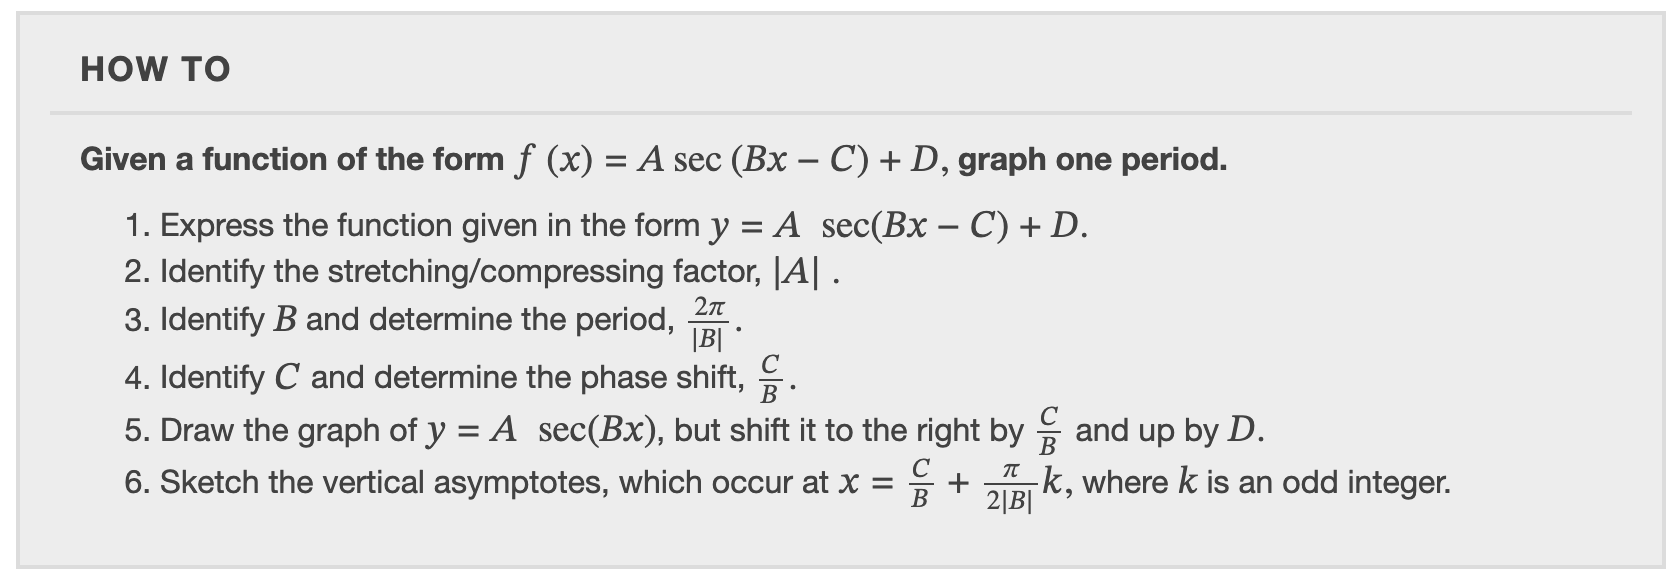
\includegraphics[width=0.9\textwidth]{./howToSec.png}
\end{center}
\end{frame}

\begin{frame}[label={sec:org19085da}]{Example}
Plot one period of the function
\[
y = 2\tan(\frac{\pi x}{4} - \frac{\pi}{2})+2\]
\vspace{10in}
\end{frame}

\begin{frame}[label={sec:org9e66205}]{Example}
\begin{center}
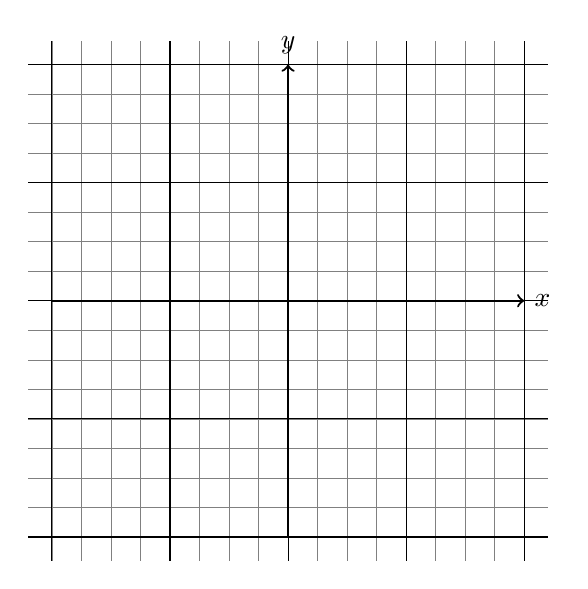
\begin{tikzpicture}[scale=3]
  \draw[help lines,step=0.125] (-1.1,-1.1) grid (1.1,1.1);
  \draw[step=0.5,thin] (-1.1,-1.1) grid (1.1,1.1);
  \draw[->,thick] (0,-1) -- (0,1) node[above] {$y$};
  \draw[->,thick] (-1,0) -- (1,0) node[right] {$x$};
\end{tikzpicture}
\end{center}
\end{frame}


\begin{frame}[label={sec:org76d414e}]{Example}
Plot one period of the function
\[
y = 2\sec \left( \frac{\pi}{4} \left( x + 1 \right) \right)\]
\vspace{10in}
\end{frame}

\begin{frame}[label={sec:org2d61f66}]{Example}
\begin{center}
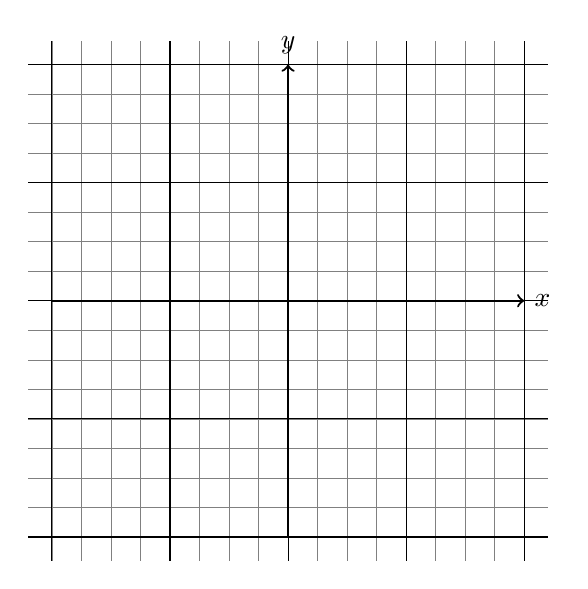
\begin{tikzpicture}[scale=3]
  \draw[help lines,step=0.125] (-1.1,-1.1) grid (1.1,1.1);
  \draw[step=0.5,thin] (-1.1,-1.1) grid (1.1,1.1);
  \draw[->,thick] (0,-1) -- (0,1) node[above] {$y$};
  \draw[->,thick] (-1,0) -- (1,0) node[right] {$x$};
\end{tikzpicture}
\end{center}
\end{frame}
\end{document}